Di dalam suatu komputer sudah pasti ada suatu mekanisme penyimpanan, contohnya
seperti memori utama yang dimiliki sistem seperti RAM (Random Access Memori).

\begin{figure}[h]
    \centering
    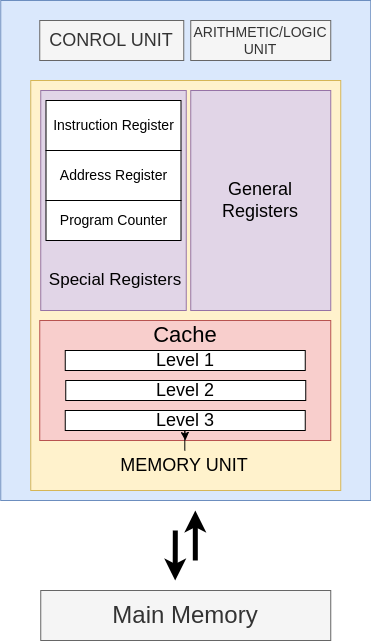
\includegraphics[scale=0.5]{MEMUNITDIAG}
    \caption{Diagram Unit Memori}
    \label{fig:MEMUNITDIAG}
\end{figure}

Namun selain RAM, CPU pun memiliki tempat penyimpanan tersendiri yang kecil didalam
chipset CPU itu sendiri, media penyimpanan tersebut disebut dengan Memori Unit.

Didalam suatu CPU, terdapat dua jenis Memori Unit yang kerap dijumpai,
yaitu Register dan juga System Cache atau CPU Cache.

Perbedaan antara Register dengan Sistem Cache terletak pada ukuran memori yang
dimiliki serta kegunaan yang mereka miliki. Berikut adalah penjelasannya.

\begin{enumerate}
  \item \textbf{Register}

    Register adalah tempat-tempat penyimpanan yang relatif berukuran kecil,
    yang terletak di dalam chipset suatu CPU.

    Karena register terletak sangat dekat dengan cpu, kecepatan dalam hal-hal
    seperti untuk read-write ke dalam memori tersebut dapat dilakukan dengan
    sangat cepat.

    Tidak ada batasan dalam berapa register yang dapat dimiliki suatu register,
    dan register dapat dibagi kedalam dua tipe bedasarkan fungsi, yaitu
    Special Register (Register Khusus), atau General Register.

    Special Register adalah register-register yang memiliki fungsi khusus yang
    sudah ditetapkan oleh rancangan suatu CPU, maka register-register ini
    berkaitan erat dengan proses-proses yang berlangsung didalam suatu CPU.

    Selain Special Register, terdapat juga General Register atau General Purpose
    Register, General Purpose Register ini adalah register-register yang tidak
    memiliki fungsi khusus dan dapat digunakan secara bebas karena tidak terikat
    dengan proses CPU.

    Special Register memiliki beberapa tipe bedasarkan fungsi atau data yang
    ia simpan, berikut adalah tipe-tipenya.

    \begin{itemize}

      \item \textbf{Current Instruction Register (CIR/IR)}

        Register yang menyimpan alamat memori dari instruksi yang
        sedang diproses.

      \item \textbf{ Program Counter Register  (PC) }

        Register yang menyimpan alamat memori selanjutnya dari suatu instruksi
        yang akan dijalankan.

      \item \textbf{Accumulator (AC)}

        Register yang menyimpan informasi terakhir dari suatu data yang diakses
        dari memori.

      \item \textbf{Memory Address Register (MAR)}

        Register yang menyimpan alamat memori yang dapat diakses jika diperlukan.

      \item \textbf{Memory Data Register (MDR) dan Memory Buffer Register (MBR)}

        Register yang menyimpan data yang akan di akses atau dikirim ke memori.

      \item \textbf{Condition Code Register}

        Register yang menyimpan status akhir dari suatu operasi.

      \item \textbf{Temporary Register}

        Register yang hanya menyimpan data-data sementara.

      \item \textbf{Input Register}

        Register yang menyimpan sebuah karakter dari input.

      \item \textbf{Input Register}

        Register yang menyimpan sebuah karakter dari ouput.

      \item \textbf{Index Register (BX)}

        Register ini menyimpan nilai dari suatu alamat memori dan merubahnya
        menjadi alamat efektif untuk digunakan dalam merubah suatu alamat dari
        data yang di operasikan.

      \item \textbf{Stack Control Registers (SCR)}

        Suatu set memori register yang berbentuk tumpukan atau \textit{stack},
        yang dalam mengakses menggunakan metode LIFO atau Last in First Out, yang
        artinya data yang pertama kali di tambahkan atau berada di tumpukan paling
        bawah hanya bisa diakses setelah telah mengakses terlebih dahulu data
        yang berada diatasnya.

      \item \textbf{Flag Register (FR)}

        Suatu set Register yang menyimpan suatu keadaan (\textit{Flag}) suatu kondisi,
        biasanya berukuran 8 bytes dengan tiap kondisi digambarkan dengan data
        atau susunan bit berukuran 8 bit.

        Ada beberapa jenis keadaan yang disimpan, yaitu.

        - \textit{Zero flags}

        - \textit{Carry flag}

        - \textit{Parity flag}

        - \textit{Sign flag}

        - \textit{Overflow flag}

      \item \textbf{Segment Register (SR)}

        Menyimpan alamat suatu memori

      \item \textbf{Data Register (DX)}

        Menyimpan alamat suatu memori suatu data yang akan dioperasikan

    \end{itemize}

    Ukuran atau besar penyimpanan sebuah register sangat beragam, tergantung
    rancangan suatu CPU, misalkan di arsitektur moderen seperti X86\_64 ukuran
    yang dimiliki suatu register berada diantara 8 bit hingga 64 bit.

    Dan batasan yang dimiliki register pun adalah salah satu penyebab suatu
    program komputer yang ditulis untuk CPU 64 bit keatas tidak bisa langsung
    dijalankan di CPU yang ber-arsitektur 32 bit tanpa dibuat suatu lapisan
    translasi yang merubah instruksi 64 bit ke dalam 32 bit.

    Register di tiap-tiap arsitektur CPU memiliki nama-nama khusus yang berguna
    untuk mengindentifikasi satu sama lainnya. Misalkan di arsitektur x86\_64
    RAX adalah label untuk sebuah General Register yang berukuran 64bit, atau
    RFLAGS yang merupakan label untuk suatu Status Register (mirip dengan Condition Register).

  \item \textbf{System Cache}

    System Cache atau CPU Cache adalah lapisan caching yang mempercepat proses
    pembacaan data dari memori utama (RAM).

    Bedasarkan Ensiklopedia Britannica, Cache atau Cache Memory adalah
    ``Memori tambahan yang secara sementara menyimpan instruksi dan data yang
    sering diakses agar dapat diproses lebih cepat oleh Central Processing Unit
    (CPU)``.

    Dalam CPU, terdapat beberapa tingkatan atau level cache, sebagaimananya dapat
    dilihat di Gambar \ref{fig:MEMUNITDIAG}. Untuk kecepatan, semakin lapisan cache
    terletak lebih dekat dengan CPU ia akan memiliki kecepatan yang lebih cepat.

    Di Gambar \ref{fig:MEMUNITDIAG}, terdapat tiga tingkatan cache sebelum
    bertemu langsung dengan RAM. Dalam mengakses data, CPU akan mulai dari lapisan tercepat,
    yaitu L1 cache atau Level 1 cache di Diagram tersebut dan ia akan mencari terus
    dari cache level 1 tersebut hingga level terakhir (L3 di diagram), dan jika data yang
    dicari belum ditemukan CPU lalu akan mencari langsung ke RAM.

    Struktur caching ini adalah penyebab kenapa sekelompok data di memory yang
    memiliki elemennya terpisah-pisah diantara suatu bongkahan memori akan lebih lambat
    untuk diakses dibanding suatu struktur data yang tersusun secara berurutan. Contoh
    dari ini adalah perbandingan antara struktur data Array dibandingkan Linked List.

\end{enumerate}
